\section{Formal Methods in Safety Analysis: A Brief History and the State of the Practice}
\label{sec:modelCheckingInSA}
Safety analysis has traditionally been performed manually, but with the rise of model checking and the improvement of its capabilities, the world of safety analysis began to see its powerful benefits~\cite{hinchey2012industrial, liggesmeyer1998improving, coudert1993fault, Bozzano:2010:DSA:1951720,bozzano2003esacs}. There arose multiple ways of viewing the system and fault models, various ways of automating the capture of safety pertinent information, and a number of tools that addressed various issues that arose. In this section, we discuss the state of the practice of related work and how formal methods has been applied in the domain of safety assessment research.

\subsection{Model Checking in Model Based Safety Analysis}
From the beginnings of model checking, there was a slow increase in its application to the domain of safety analysis, but a few research groups contributed immensely to this branch of study. Separately, these researchers began to contribute to safety analysis through the use of formal methods in the '90s and are still contributing today (e.g., \cite{reese1997software,signoret1998altarica,chiappini1999formal,cimatti2000industrial}. 

One of the main methods was the abstraction of the system into a formal transition system; this provided a means of defining a precise mathematical model of the system and simplifying mathematical operations through the use of abstraction techniques on the transition system. This helped to shrink the entire state space into something more digestible by computational techniques~\cite{d2008survey}. 

In the early 2000s, model based safety assessment began to make an appearance in literature~\cite{Bozzano:2010:DSA:1951720,Joshi05:Dasc, Joshi05:SafeComp, Joshi07:Hase}. The researchers began applied model checking in model based system development to safety analysis.  In this approach, a safety analysis system model is the central artifact in the safety analysis process, and traditional safety analysis artifacts, such as fault trees, are automatically generated by tools that analyze the system model.

The contents and structure of the safety analysis system model differ significantly across different conceptions of model-based safety analysis.  We can draw distinctions between approaches along several different axes.  The first is whether they propagate errors explicitly through user-defined propagations, which we call {\em explicit propagation}, or through behavioral requirements and interactions in the model itself, which we call {\em implicit propagation}.  The next is whether models and notations are {\em purpose-built} for safety analysis vs. those that extend {\em existing system models}.

For implicit propagation approaches, there are several additional dimensions.  One dimension involves whether {\em causal} or {\em non-causal} models are allowed.  Non-causal models allow simultaneous (in time) bi-directional error propagations, which allow more natural expression of some failure types (e.g. reverse flow within segments of a pipe), but are more difficult to analyze.  A final dimension involves whether analysis is {\em compositional} across layers of hierarchically-composed systems or {\em monolithic}.  

\begin{figure}[h]
	\begin{center}
		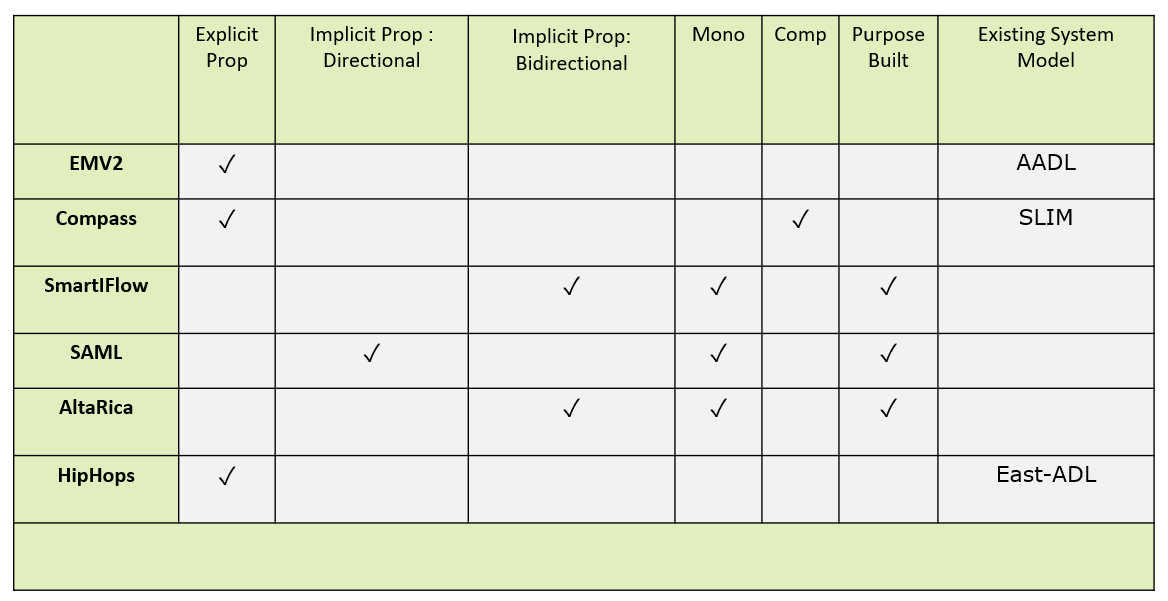
\includegraphics[width=\textwidth]{images/relatedWork.PNG}
	\end{center}
	\caption{Approaches of Related Work}
	\label{fig:relatedWork}
\end{figure}

Figure~\ref{fig:relatedWork} highlights the differences between these approaches in closely related work. The left column of the figure shows the tool names and across the top row are the various ways of structuring and analyzing the safety analysis system model. The tools and their approaches are described in the following subsections. 

These tools attempt to address various needs in the safety community and do so in distinct ways, but we wish to combine many of these efforts under one existing system model. We make it possible to extend the AADL system model with a fault model. Both nominal and fault analysis should be able to be performed monolithically or compositionally, and the fault model should allow for either explicit or implicit propagation. We attempt to address multiple needs within a single framework, unlike many of the related tools. 

To summarize, we created a safety modeling framework that allows for (1) both {\em implicit} and {\em explicit} directional propagation, (2) both {\em monolithic} and {\em compositional} verification, and (3) that extends an existing system model. 

The following literature overview is not a complete account of all safety analysis model checking tools available either in industry or research, but highlights some of the most influential and closely related safety assessment methods and tools currently available. 

\subsubsection{AltaRica}
AltaRica was one of the first model checking tools specifically aimed at safety analysis of critical systems. The first iteration of AltaRica (1.0) performed over a transition system of the model, used dataflow ({\em causal}) semantics, and could capture the hierarchy of a system~\cite{signoret1998altarica}. The key idea was that this transition system (more specifically {\em constraint automata}) could be compiled into Boolean formulae and transformed into a binary decision diagram~\cite{point1999altarica}. The literature for performing fault tree analysis over BDDs was rich with algorithms; this was how much of the safety analysis artifacts were generated. The dataflow dialect (AltaRica 1.0) has substantial tool support, including the commercial Cecilia OCAS tool from Dassault~\cite{bieber2004safety}. For this dialect, the safety assessment, fault tree generation, and functional verification can be performed with the aid of NuSMV model checking~\cite{symbAltaRica}.

The most recent language update (AltaRica 3.0) uses non-causal semantics~\cite{prosvirnova2013compilationfaulttrees,prosvirnova2015automated,PROSVIRNOVA2013127}. Failure states are defined throughout the system and flow variables are updated through the use of assertions~\cite{Bieber04safetyassessment}.  AltaRica 3.0 has support for simulation and Markov model generation through the OpenAltaRica (www.openaltarica.fr) tool suite; it uses {\em implicit error propagation}, and it is a {\em purpose-built}, {\em monolithic} safety analysis language. 

\subsubsection{FSAP, xSAP, and COMPASS}
The Formal Safety Analysis Platform (FSAP) was introduced in 2003~\cite{bozzano2003improving} and supported failure mode definitions, safety requirements in temporal logic formulae, automated fault tree construction, and counterexample traces. The platform used NuSMV, a binary decision diagram (BDD)-based model checker~\cite{Cimatti2000}. The system model, written in NuSMV, and the fault model, developed graphically in FSAP, are together translated into a finite state machine and eventually into a BDD; fault tree analysis is performed using BDD algorithms implemented in NuSMV. 

By 2016, the researchers that developed FSAP (Foundation Bruno Kessler, FBK) released a similar tool called xSAP~\cite{DBLP:conf/tacas/BittnerBCCGGMMZ16}. xSAP extends FSAP in many ways: xSAP can handle infinite state machines, it is textual language rather than graphical, allows for richer fault modeling and definitions, and implements more than just BDD computations (e.g., SAT- and SMT-based routines). xSAP was integrated into the COMPASS toolsuite to take advantage of the algorithms it supports. More complex SAT-based algorithms were introduced to bypass the BDD method of minimal cut set generation, namely the ``anytime approximation" algorithms~\cite{CAV2015:BoCiGrMa, mattarei2016scalable}. These algorithms make clever use of bounded model checking algorithms to explore counterexamples provided to the query "the top level event never occurs." These explorations are done such that the cut sets generated are of increasing cardinality which allows for an approximation computation to be given even when the state space is too large to compute all minimal cut sets. These are implemented in xSAP~\cite{CAV2015:BoCiGrMa}.

COMPASS (Correctness, Modeling project and Performance of Aerospace Systems)~\cite{10.1007/978-3-642-04468-7_15} allows for {\em explicit propagation}, and is a {\em causal} {\em compositional} tool suite that uses the SLIM language, which is based on a subset of the Architecture Analysis and Design Language (AADL), for its input models~\cite{5185388, criticalembeddedsystems}. In SLIM, a nominal system model and the error model are developed separately and then transformed into an extended system model.  This extended model is automatically translated into input models for the NuSMV model checker~\cite{Cimatti2000, NuSMV}, MRMC (Markov Reward Model Checker)~\cite{Katoen:2005:MRM:1114692.1115230, MRMC}, and RAT (Requirements Analysis Tool)~\cite{RAT}. The safety analysis tool xSAP~\cite{DBLP:conf/tacas/BittnerBCCGGMMZ16} can be invoked in order to generate safety analysis artifacts such as fault trees and FMEA tables~\cite{compass30toolset}.  %COMPASS is an impressive tool suite, but some of the features that make AADL suitable for SW/HW architecture specification: event and event-data ports, threads, and processes, appear to be missing, which means that the SLIM language may not be suitable as a general system design notation (ESM).

\subsubsection{SmartIFlow}
SmartIFlow~\cite{info17:HaLuHo,honig2014new} uses {\em implicit propagation} and is a {\em purpose-built}, {\em monolithic} {\em non-causal} safety analysis tool that describes components and their interactions using finite state machines and events. Verification is done through an explicit state model checker which returns sets of counterexamples for safety requirements in the presence of failures.  SmartIFlow allows {\em non-causal} models containing simultaneous (in time) bi-directional error propagations.  On the other hand, the tools do not yet appear to scale to industrial-sized problems, as mentioned by the authors: ``As current experience is based on models with limited size, there is still a long way to go to make this approach ready for application in an industrial context''~\cite{info17:HaLuHo}.

\subsubsection{SAML}
The Safety Analysis and Modeling Language (SAML)~\cite{Gudemann:2010:FQQ:1909626.1909813} uses {\em implicit propagation}, and is a {\em purpose-built}, {\em monolithic} {\em causal} safety analysis language that was developed in 2010.  System models constructed in SAML can be used used for both qualitative and quantitative analyses. It allows for the combination of discrete probability distributions and non-determinism. The SAML model can be automatically imported into several analysis tools like NuSMV~\cite{Cimatti2000}, PRISM (Probabilistic Symbolic Model Checker)~\cite{CAV2011:KwNoPa}, or the MRMC model checker~\cite{Katoen:2005:MRM:1114692.1115230}. SAML itself does not provide the formal verification engines, but instead provides a platform to model the safety aspects of a system and then translate this into the input language for a formal verification engine~\cite{Gudemann:2010:FQQ:1909626.1909813}.

\subsubsection{Error Model Annex for AADL}
The SAE (Society of Automotive Engineers) released the
aerospace standard AS5506, named Architecture Analysis and Design Language (AADL), which is a mature industry-standard for embedded systems and has proved to be efficient for architecture modeling~\cite{aerospace2012sae,liu2016research}. AADL supports safety analysis by adding EMA (Error Model Annex) as an extension to the language. EMA allows the user to annotate system hardware and software architectures with hazard, error propagation, failure modes and effects due to failures. Around 2016, Version 2 of the Error Model Annex was released (EMV2)~\cite{EMV2}. EMV2 uses {\em explicit propagation} and is based on an {\em existing system model} approach. The faults and error propagations are explicitly defined and the fault tree analysis is performed by traversing propagation paths in reverse to find the original fault that caused the problem~\cite{feiler2017automated}. 


